\subsection{Integration of the Radiation Transfer Equation}

\begin{figure}[ht]
	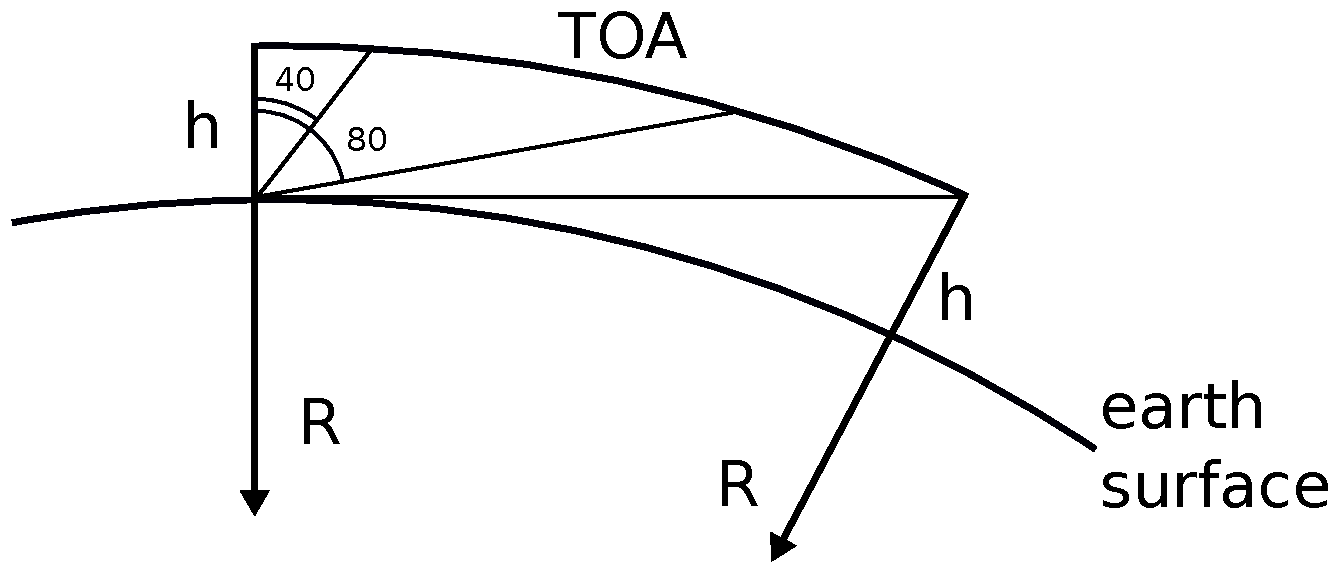
\includegraphics[width=12cm]{figures/earth_surface_toa.pdf}
	\caption{Geometry of earth and atmosphere}
	\label{fig:geometry}
\end{figure}

The intensity in \eqn{eqn1} is integrated along a path from the earth surface to the TOA (top of atmosphere) which is assumed to be at a height of $70\; km$. Assuming constant $\kappa$ and $\epsilon$ in \eqn{eqn1} the solution is given by:
\begin{align}
	I(\lambda,z) &= I(\lambda,z_0) \exp( -  \kappa(\lambda) (z-z_0)) + \dfrac{\epsilon(\lambda)}{\kappa(\lambda)} \left(1 - \exp( - \kappa(\lambda) (z-z_0))\right)
\end{align}
Because $\kappa$ and $\epsilon$ are not constant along the path from earths surface to TOA the integration is subdivided into many steps. At each step $\kappa$ and $\epsilon$ are calculated using local values of temperature and density.
\newline

In order to compute the total irradiance emanating from an area element of the surface to TOA the integration has to be done over the half sphere (\fig{fig:geometry}):
\begin{align}
	F &= \int_0^{2 \pi} \int_0^{\pi/2} I(\theta) \sin(\theta) \cos(\theta)  d \theta d \phi \\
	  &= 2 \pi \int_0^{\pi/2} I(\theta) \sin(\theta) \cos(\theta) d \theta
\end{align}
The intensity $I(\theta)$ is computed at $\theta_1=0^o, \theta_2=40^o, \theta_3=40^o$.
The intermediate values are interpolated by a cubic polynomial (see \chap{app_a_2}):
\begin{align}
	I(\theta) = I(\theta=0) + a_2 \theta_2^2 + a_3 \theta_3^3
\end{align}
The term linear in $\theta$ is zero because of $\dfrac{d T(\theta)}{d\theta}|_{(\theta=\theta_1)} = 0$.
\newline

The polynomial coefficients can be determined analytically:
\begin{align}
	a_2 &= \dfrac{( I(\theta_2) - I(\theta_1) ) \theta_3^3 - (I(\theta_3) - I(\theta_1)) \theta_2^3}{\theta_1^2 \theta_2^3 - \theta_1^3 \theta_2^2} \\
	a_3 &= \dfrac{( I(\theta_3) - I(\theta_1) ) \theta_2^2 - (I(\theta_2) - I(\theta_1)) \theta_3^2}{\theta_1^2 \theta_2^3 - \theta_1^3 \theta_2^2}
 \end{align}
With this the integral is given by:
\begin{align}
	F &= 2 \pi \int_0^{\pi/2} \left(I(0) + a_2 \theta^2 + a_3 \theta^3\right) \sin(\theta) \cos(\theta)  d \theta
\end{align}
The contributions of the different polynomial orders assuming $I(\theta) = 1$ are:
\begin{align*}
	 &\int_0^{\pi/2} \sin(\theta) \cos(\theta) d \theta = 0.5 \\
	 &\int_0^{\pi/2} \theta^2 \sin(\theta) \cos(\theta) d \theta = 0.37  \\
	 &\int_0^{\pi/2} \theta^3 \sin(\theta) \cos(\theta) d \theta = 0.38
\end{align*}

\subsection{The HITRAN Data}

The spectroscopic $\mathrm{CO}_2$ data where taken from the HITRAN database (\cite{hitran1}). The standard HITRAN data files use a fixed size format and include data that are not used in the present model. HITRAN allows to define ones own format and data output. For easier handling the entries are separated by commas. The data rows are composed of:
\begin{enumerate}
	\item Molecule ID, for $\mathrm{CO}_2$ this is $2$
 	\item Isotopologue ID, for $\mathrm{CO}_2$ $1-9$
 	\item The transition wavenumber $\nu$	[$cm^{-1}$]
    \item The line strength multiplied by isotopologue abundance $S$, [$cm^{-1}/(\mathrm{mole} \;cm^{-2}$)]
 	\item Einstein coefficient of spontaneous emission $A$ [$s^{-1}$]
 	\item Pressure line broadening coefficient by collisions with air molecules $\gamma_{air}$ [$cm^{-1} atm^{-1}$]
 	\item pressure line broadening coefficient by collisions with $\mathrm{CO}_2$ molecules $\gamma_{self}$ [$cm^{-1} atm^{-1}$]
	\item Energy of the lower state $E_l$ [$cm^{-1}$]
	\item Temperature exponent $n_{air}$ for the air broadened HWHM
	\item Pressure shift induced by air (pressure) $\delta_{air}$, referred to $p = 1\; atm$ [$cm^{-1} atm^{-1}$]
	\item Upper state degeneracy $g_u$
	\item Lower state degeneracy $g_l$
\end{enumerate}
In the present report wavelength unit is meter and energy unit is Joule, whereas HITRAN uses wavenumber [$cm^{-1}$]. The transition from wavelength to wavenumber has to be done carefully.
\begin{align*}
	\lambda_{ul}     & \leftarrow \dfrac{10^{-2}}{\nu}               & [m]                   \\
	\Delta E_{ul}    & \leftarrow \dfrac{h  c}{\lambda_{ul}}         & [J]                   \\
 	E_l              & \leftarrow h  c  \dfrac{E_l}{10^{-2}}         & [J]                   \\
	E_u              & \leftarrow E_l + \Delta E_{ul}                  & [J]                   \\
	\gamma_a         & \leftarrow \dfrac{\gamma_{air}}{10^{-2}}  10^{-5} & \left[\dfrac{1}{m \; Pa}\right] \\
	\gamma_s         & \leftarrow \dfrac{\gamma_{self}}{10^{-2}}  10^{-5} & \left[\dfrac{1}{m \; Pa}\right] \\
	\delta_a         & \leftarrow \dfrac{\delta_{air}}{10^{-2}}  10^{-5} &
\end{align*}

The Gauss profile is given as:
\begin{align*}
	g_G(\nu;\nu_{ij}, T) = \sqrt{\dfrac{\ln 2}{\pi \alpha_D^2}} \exp\left(- \dfrac{(\nu - \nu_{ij})^2}{\alpha_D^2}\right)
\end{align*}
with the HWHM Doppler line broadening:
\begin{align*}
	\alpha_D(T) = \dfrac{\nu_{ij}}{c} \sqrt{\dfrac{2 N_A k_B T \ln 2}{M}}
\end{align*}
$N_A$ is the Avogadro constant and $M_{mole}$ is the molar mass of the isotopologue.
\newline

The Lorentz profile is given by HITRAN as \cite{hitran2}:
\begin{align*}
	g_G(\nu;\nu_{ij}, T) \dfrac{1}{\pi} \dfrac{\gamma(p,T)}{\gamma(p,T)^2 + \left[ \nu - (\nu_{ij} + \delta(p_{ref})^2\right]}
\end{align*}
with the temperature and pressure dependence of pressure broadened line width and pressure shift:
\begin{align*}
	\gamma(p, T) &= \left(\dfrac{T_{ref}}{T}\right)^{n_{air}}
	               \left(  \gamma_{air} (p_{ref}, T_{ref}) (p - p_{self}) +
	                       \gamma_{self}(p_{ref}, T_{ref}) p_{self}  \right) 		 \\
	\nu_{ij}^*   &= \nu_{ij} \delta(p_{ref}) p
\end{align*}
Temperature dependent partition functions for $\mathrm{CO}_2$ can be found at \cite{hitran3}.

\subsection{Computational Details}

The wavelength dependent intensity and the absorption and emission coefficients are discretized between $13 \mu m$ and $17 \mu m$. The wavelength resolution used is $10^{-11} m$. In order to check if this resolution is sufficient computations with $10^{-12} m$ were performed but showed only very small differences compared to the coarser resolution.
\newline
\newline
The initial intensity is given by the Planck function at $288 K$:
\begin{align}
	I_\lambda = \dfrac{2 \pi h c^2}{\lambda^5} \dfrac{1}{\exp\left(\dfrac{h c}{\lambda k_B T}\right) - 1}
\end{align}
The absorption and emission coefficients are the sums of all contributing lines:
\begin{align*}
	\kappa(\lambda_i)   &= \sum_j \kappa_j   f_j(\lambda_i - \lambda_j) \\
	\epsilon(\lambda_i) &= \sum_j \epsilon_j f_j(\lambda_i - \lambda_j)
\end{align*}
$i$ is the wavelength index of the descretized wavelength and $j$ is the line index.


